% =============================================================================
% Track 2 (High Performance Computing) manuscript -- INDIACom 2027
% DRAFT 1, 2026-11-05. Supersedes the control-focused main.tex for this submission.
%
% RULES FOR THIS FILE
%  * Every measured number comes from a macro defined in numbers_track2.tex, which is
%    GENERATED from the raw CSVs by scripts/make_paper_numbers.py. Nothing measured is typed
%    here by hand. A macro that has not been generated yet prints as a red TODO.
%  * Page limit, template and Track 2 scope are NOT yet confirmed (official call text needed).
%  * Build:  pdflatex main_track2 && bibtex main_track2 && pdflatex main_track2 && pdflatex main_track2
% =============================================================================
\documentclass[conference]{IEEEtran}
\IEEEoverridecommandlockouts

\usepackage{cite}
\usepackage{amsmath,amssymb}
\usepackage{graphicx}
\usepackage{booktabs}
\usepackage{siunitx}
\DeclareSIUnit{\year}{yr}
\DeclareSIUnit{\day}{d}
\usepackage[hidelinks]{hyperref}
\usepackage{xcolor}

\graphicspath{{figures/}{../results/figures/}}
\newcommand{\TODO}[1]{\textcolor{red}{[\textbf{TODO:} #1]}}
\newcommand{\dVdeg}{\Delta V_{\mathrm{deg}}}

% ---- measured numbers: generated file first, then red fallbacks for anything missing ----
\IfFileExists{numbers_track2.tex}{% GENERATED by scripts/make_paper_numbers.py -- do not edit by hand.
\newcommand{\NumSimOne}{\num{12300}}
\newcommand{\NumSimDaysPerSecOne}{8.5}
\newcommand{\NumSimEight}{\num{69800}}
\newcommand{\NumSpeedEight}{5.7}
\newcommand{\NumEffEight}{0.71}
\newcommand{\NumSimSixteen}{\num{75800}}
\newcommand{\NumSpeedSixteen}{6.2}
\newcommand{\NumEffSixteen}{0.39}
\newcommand{\NumSmtTwo}{1.13}
\newcommand{\NumSmtGain}{8.6}
\newcommand{\NumSimDaysPerSecMax}{53}
\newcommand{\NumYearSeconds}{6.9}
\newcommand{\NumFreqOneGHz}{5.0}
\newcommand{\NumFreqEightGHz}{3.7}
\newcommand{\NumPerWorkerOne}{\num{12500}}
\newcommand{\NumPerWorkerEight}{\num{9110}}
\newcommand{\NumPerGhzRatioEight}{0.98}
\newcommand{\NumSlowFastSameWork}{1.03}
\newcommand{\NumGridUnits}{84}
\newcommand{\NumGridSteps}{\num{8709120}}
\newcommand{\NumGridSeconds}{223}
\newcommand{\NumGridWorkers}{6}
\newcommand{\NumGridDaysPerSec}{27}
\newcommand{\NumLifeMin}{1.2}
\newcommand{\NumLifeMax}{19}
\newcommand{\NumLifeSpread}{16}
\newcommand{\NumLifeNominalNaive}{5.0}
\newcommand{\NumLifeNominalRamp}{6.2}
\newcommand{\NumLifeNominalNoThr}{5.9}
\newcommand{\NumRankFlips}{6}
\newcommand{\NumVariants}{13}
\newcommand{\NumScenLifeMin}{3.4}
\newcommand{\NumScenLifeMax}{6.9}
\newcommand{\NumScenHydrogenSpreadPct}{4.4}
\newcommand{\NumGpuUps}{\num{171}}
\newcommand{\NumCpuUpsFour}{\num{98}}
\newcommand{\NumCpuUpsEight}{\num{110}}
\newcommand{\NumGpuCpuRatio}{1.6}
\newcommand{\NumMultiGpuOne}{\num{180}}
\newcommand{\NumMultiGpuTwo}{\num{255}}
\newcommand{\NumMultiGpuFour}{\num{330}}
\newcommand{\NumMultiCpuOne}{\num{100}}
\newcommand{\NumMultiCpuFour}{\num{180}}
\newcommand{\NumMultiMixed}{\num{272}}
\newcommand{\NumMultiBest}{\num{330}}
\newcommand{\NumMultiBestCase}{\texttt{gpu\_x4}}
}{}
\providecommand{\NumSimOne}{\TODO{sim 1-core steps/s}}
\providecommand{\NumSimEight}{\TODO{sim 8-worker steps/s}}
\providecommand{\NumSimSixteen}{\TODO{sim 16-worker steps/s}}
\providecommand{\NumSpeedEight}{\TODO{S(8)}}
\providecommand{\NumEffEight}{\TODO{E(8)}}
\providecommand{\NumSpeedSixteen}{\TODO{S(16)}}
\providecommand{\NumEffSixteen}{\TODO{E(16)}}
\providecommand{\NumSimDaysPerSecOne}{\TODO{sim days/s, 1 core}}
\providecommand{\NumSimDaysPerSecMax}{\TODO{sim days/s, max}}
\providecommand{\NumYearSeconds}{\TODO{seconds per simulated year}}
\providecommand{\NumGpuUps}{\TODO{GPU updates/s}}
\providecommand{\NumCpuUpsFour}{\TODO{CPU(4) updates/s}}
\providecommand{\NumCpuUpsEight}{\TODO{CPU(8) updates/s}}
\providecommand{\NumGpuCpuRatio}{\TODO{GPU/CPU ratio}}
\providecommand{\NumSmtTwo}{\TODO{S(2) on one SMT pair}}
\providecommand{\NumSmtGain}{\TODO{gain of 16 over 8 workers, \%}}
\providecommand{\NumFreqOneGHz}{\TODO{clock at 1 worker}}
\providecommand{\NumFreqEightGHz}{\TODO{clock at 8 workers}}
\providecommand{\NumPerWorkerOne}{\TODO{per-worker rate, 1 worker}}
\providecommand{\NumPerWorkerEight}{\TODO{per-worker rate, 8 workers}}
\providecommand{\NumPerGhzRatioEight}{\TODO{rate-per-GHz ratio}}
\providecommand{\NumSlowFastSameWork}{\TODO{slowest/fastest worker}}
\providecommand{\NumGridUnits}{\TODO{grid units}}
\providecommand{\NumGridSteps}{\TODO{grid env steps}}
\providecommand{\NumGridSeconds}{\TODO{grid seconds}}
\providecommand{\NumGridWorkers}{\TODO{grid workers}}
\providecommand{\NumGridDaysPerSec}{\TODO{grid simulated days/s}}
\providecommand{\NumLifeMin}{\TODO{life min}}
\providecommand{\NumLifeMax}{\TODO{life max}}
\providecommand{\NumLifeSpread}{\TODO{life spread}}
\providecommand{\NumLifeNominalNaive}{\TODO{nominal life, published rule}}
\providecommand{\NumLifeNominalRamp}{\TODO{nominal life, slew limit}}
\providecommand{\NumLifeNominalNoThr}{\TODO{nominal life, no threshold}}
\providecommand{\NumRankFlips}{\TODO{rank flips}}
\providecommand{\NumVariants}{\TODO{variants}}
\providecommand{\NumScenLifeMin}{\TODO{scenario life min}}
\providecommand{\NumScenLifeMax}{\TODO{scenario life max}}
\providecommand{\NumScenHydrogenSpreadPct}{\TODO{scenario H2 spread}}
\providecommand{\NumMultiGpuOne}{\TODO{GPU x1 aggregate}}
\providecommand{\NumMultiGpuTwo}{\TODO{GPU x2 aggregate}}
\providecommand{\NumMultiGpuFour}{\TODO{GPU x4 aggregate}}
\providecommand{\NumMultiCpuOne}{\TODO{CPU x1 aggregate}}
\providecommand{\NumMultiCpuFour}{\TODO{CPU x4 aggregate}}
\providecommand{\NumMultiMixed}{\TODO{mixed aggregate}}
\providecommand{\NumMultiBest}{\TODO{best aggregate updates/s}}
\providecommand{\NumMultiBestCase}{\TODO{best concurrency case}}

\begin{document}

\title{Simulation Throughput and Learner Scaling for Reinforcement-Learning Control of a PEM
Electrolyzer under Variable Renewable Input: A Computational Performance Study}

\author{\IEEEauthorblockN{\TODO{authors}}
\IEEEauthorblockA{\TODO{affiliation}}}

\maketitle

% =============================================================================
\begin{abstract}
Degradation of proton-exchange-membrane (PEM) electrolyzer stacks unfolds over years, so control
strategies for renewable-powered operation must be screened in simulation long before any
hardware test is possible. We study the computational side of that screening for a
\SI{1}{\mega\watt}-class plant simulated at a one-minute control interval. On a single
workstation (8 cores, one GPU) the simulator runs at \NumSimOne{} environment steps/s on one core
and \NumSimSixteen{} steps/s with 16 workers, i.e.\ \NumYearSeconds{} s of wall time per
simulated year; scaling is limited by the 8 physical cores (speedup \NumSpeedEight{} on 8
workers). Soft Actor-Critic (SAC) training at a correct update-to-data ratio is
learner-bound at \NumGpuUps{} updates/s on the GPU and \NumCpuUpsFour{}--\NumCpuUpsEight{} on
the CPU, independent of the number of environments. We also report a measurement pitfall: a
vectorized SAC configuration documented as one gradient update per transition performed
$0.032$, so speedups quoted in steps/s overstated learning throughput by about $30\times$. We
therefore compare configurations by time to a stated quality at a stated update ratio.
\TODO{one sentence on the learned-controller outcome once experiments E3--E5 are final} No
physical stack was operated: the simulator is a pre-screening tool, and conclusions concern
relative controller behaviour and computational performance, not absolute stack lifetime.
\end{abstract}

\begin{IEEEkeywords}
PEM water electrolysis, reinforcement learning, parallel simulation, scaling analysis,
update-to-data ratio, performance benchmarking
\end{IEEEkeywords}

% =============================================================================
\section{Introduction}
Green hydrogen from variable renewable generation depends on electrolyzer stacks that last. In
PEM electrolyzers, degradation accumulates over years and is driven in part by \emph{how} the
stack is operated: frequent load fluctuations during dynamic operation are reported to accelerate
it~\cite{sayedahmed2024dynamic}. The specific mechanisms we model, start--stop cycling and fast ramps,
are attributed to intermittent supply in~\cite{intermittency2025}
\TODO{that reference could not be found by title; verify before submission}. A physical test of one control strategy therefore takes a
substantial fraction of a stack's life, and cannot explore the combinations of resource
variability and degradation parameters a designer needs to examine. Simulation is the only
practical way to screen strategies, and its usefulness is set by two computational questions:
how fast can the plant and its operating environment be simulated, and what does it cost to
train a learning-based controller against that simulator?

We address both for a \SI{1}{\mega\watt}-class PEM electrolyzer powered directly by a hybrid
solar--wind resource at a one-minute control interval, a setting in which the control problem is
cheap per step but needs very many steps. Our contributions are measurements and one
correction, not a new algorithm:

\begin{itemize}
  \item \textbf{Simulator scaling.} Throughput and parallel efficiency of the plant simulator as a
        function of worker count, with worker placement (one per physical core, packed on
        hyper-thread pairs, or left to the operating system) controlled and reported.
  \item \textbf{Learner scaling.} Where SAC training time actually goes at a correct
        update-to-data ratio: CPU against GPU, the effect of batch size, and the aggregate
        throughput of several concurrent runs on one machine.
  \item \textbf{A benchmarking pitfall.} We show that a documented one-update-per-transition SAC
        configuration with vectorized environments in Stable-Baselines3 performed one update per
        32 transitions, and that throughput in steps/s is therefore not comparable across update
        ratios.
  \item \textbf{Parallel sensitivity analysis.} A parameterised renewable-variability generator and a
        process-parallel evaluation harness for controller comparison under uncertainty in
        both the resource and the degradation coefficients.
  \item \textbf{An honest controller comparison.} \TODO{finalise after E3--E5}
\end{itemize}

\emph{Scope.} This is a simulation study. No physical stack was operated, the degradation model
is calibrated to literature-reported rates rather than measured, and the sub-hourly resource
variability is synthetic. The value claimed for the simulator is rapid pre-screening and
what-if analysis; hardware validation is future work (Section~\ref{sec:limits}).

% =============================================================================
\section{Related Work}
\emph{Degradation and control.} Degradation mechanisms of PEM water electrolysis are
reviewed in~\cite{feng2017pemwe,bernhardt2026degradation}, and the specific effect of
renewable intermittency (cycling, ohmic resistance rise, thermal fatigue) is surveyed
in~\cite{intermittency2025} \TODO{unverified: not found by title; see refs.bib}. A review of
degradation models for power allocation and energy management is given in~\cite{degmodels2025}
\TODO{existence verified; the specific rates we rely on are not}. Reinforcement learning has been applied to alkaline electrolysis under renewable
input~\cite{awe_rl_2025} and to PEM scheduling~\cite{drl_scheduling_2026}; neither uses a
one-minute control interval with an explicit degradation term. \TODO{reference status:
see audit/01\_research\_audit.md, C5}

\emph{Parallel simulation for RL.} Environment execution is often the slowest part of an RL
system, and engines that run many environments in parallel have been built for that
reason~\cite{weng2022envpool}. Our simulator is a small pure-Python model, so we study process-level
parallelism rather than a native engine.

\emph{Update-to-data ratio.} The number of gradient updates per collected transition (the replay
ratio or update-to-data ratio) is a first-order determinant of off-policy performance and is
treated as an explicit variable in the literature~\cite{fedus2020replay,chen2021redq,doro2023replay}.
Comparing training speeds between configurations that differ in this ratio compares different
amounts of learning work; this is the pitfall we document in Section~\ref{sec:utd}.

% =============================================================================
\section{Workload: Plant, Degradation and Control Problem}\label{sec:workload}
\subsection{Plant}
The plant has 280 cells of \SI{1000}{\centi\meter\squared}, rated at
$j_\mathrm{r}=\SI{2.0}{\ampere\per\centi\meter\squared}$ and \SI{60}{\celsius}, with the cathode
at \SI{30}{\bar}. Cell voltage is the sum of a reversible term with a Nernst pressure
correction, Butler--Volmer activation losses at both electrodes, ohmic loss, a
concentration term and the degradation state,
\begin{equation}
V_\mathrm{cell}(j)=E_\mathrm{rev}(T,p)+V_\mathrm{act}(j)+V_\mathrm{ohm}(j)+V_\mathrm{conc}(j)+\dVdeg .
\label{eq:vcell}
\end{equation}
Hydrogen production follows Faraday's law derated by a Faradaic efficiency
$1-j_\mathrm{cross}/j$, where the crossover current density follows from Fick's law and the
membrane thickness. A constant balance-of-plant load of \SI{1.5}{\percent} of rated is drawn
whenever the stack is on; rated plant power is \SI{1049}{\kilo\watt} and the plant cannot run below
\SI{36.8}{\kilo\watt}. The model reproduces the cell voltage at the stated current densities
(\SI{1.507}{\volt} at \SI{0.05}{\ampere\per\centi\meter\squared} and \SI{1.846}{\volt} at rated).
The model is parameterised from published ranges and is not fitted to a device.

\subsection{Degradation}
Degradation is a scalar cell-voltage rise $\dVdeg$ in microvolts, entering~\eqref{eq:vcell}. Five
terms add per step: a base rate while on, a high-current term
$k_j\max(0,j/j_\mathrm{r}-0.6)^2$, a ramp term $k_r|\mathrm{d}j/\mathrm{d}t|$, a fixed cost per on/off
transition, and an idle rate while off. The coefficients ($r_\mathrm{base}=1.75$,
$k_j=20$, $k_r=31$, $\Delta V_\mathrm{cycle}=1.0$, $r_\mathrm{idle}=0.75$, in
\si{\micro\volt} and \si{\micro\volt\per\hour} units as appropriate) were solved so that a
published load-following rule reproduces a literature stack life of about five years. The
absolute scale is therefore anchored to a single published figure \TODO{anchor reference not yet
verified against full text} and we report \emph{relative} comparisons only.

\subsection{Control problem}
Control is a Markov decision process with $\Delta t=\SI{1}{\minute}$ and a one-day
episode ($T=1440$ steps). The action is a scalar $a_t\in[-1,1]$ mapped to a fraction
$u_t=\tfrac12(a_t+1)$ of the \emph{currently available} renewable power, so the setpoint
never exceeds the resource (renewable-only operation). The eight-dimensional observation holds
the available power, its 15-minute mean, the previous setpoint, current density, normalised
degradation, hydrogen rate and the time of day. The reward is
$r_t=w_1\tilde m_{\mathrm{H_2}}-w_2\widetilde{\dVdeg}-w_3|\Delta j|/j_\mathrm{r}$ with fixed scales;
$w_2$ is swept to trace a yield--degradation frontier. Because the learned policy is trained on
independent days with the degradation state reset, the agent receives degradation information
through the reward only.

\subsection{Resource and baselines}
The resource is ERA5 hourly data~\cite{hersbach2020era5} for Kutch, Gujarat (2019), converted
with a PVWatts-style PV model~\cite{dobos2014pvwatts} and a turbine power curve (both ours), and
upsampled to one minute with Ornstein--Uhlenbeck noise that preserves each hourly mean
exactly; \num{293} days train and \num{72} are held out. The hybrid input averages
\SI{42}{\percent} of the plant rating. Because no measured one-minute data are available here, the
noise amplitudes are assumptions; Section~\ref{sec:scen} varies them. Controllers compared are
the published load-following rule with a \SI{10}{\percent} idle threshold~\cite{pvt_control_2026}
\TODO{verify that this source states this rule}, the same rule without the threshold (a constant
action of $+1$), and a tuned slew-rate-limited rule.

% =============================================================================
\section{Computational Methodology}\label{sec:method}
\subsection{Simulator and parallelism}
One environment step maps the commanded power to a current density, evaluates the polarisation
model, and updates the degradation state. The inversion from power to current density,
originally a bisection, uses a table of the zero-degradation power curve (4096 points) with
linear interpolation and two fixed-point corrections for the degradation term. We parallelise
across independent episodes in separate processes; there is no shared state between workers.

\subsection{Simulator benchmark protocol}
Workers run random-action episodes of the bare environment (no policy, no SB3). Each worker builds its
environment and takes warm-up steps, then all workers pass a barrier; timing starts at the
barrier and ends when the last worker finishes. We report \emph{strong scaling} (fixed total
work of 64 episodes, \num{92160} steps, split over $n$ workers), giving $S(n)=T(1)/T(n)$ and
$E(n)=S(n)/n$, and \emph{weak scaling} (8 episodes per worker). Placement is varied:
unpinned (the operating system decides), pinned one worker per physical core, and pinned
onto hyper-thread sibling pairs. Each case is repeated; we show bootstrap intervals over
repeats, which characterise run-to-run variation on this machine only.

\subsection{Learner benchmark protocol}
We time \texttt{model.train()} on a replay buffer already filled past the learning-start
threshold, so environment stepping is excluded and the number is the learner's ceiling.
Variables are device, batch size, and CPU thread count. For concurrency, $k$ independent
learner processes build their models, wait for a common wall-clock start, and are timed over
an overlapping window; the aggregate rate is total updates over the span from the first start to the
last finish.

\subsection{Update-to-data accounting}\label{sec:utd}
Let $N$ be the number of vectorized environments, $F$ the \texttt{train\_freq} and $G$ the
\texttt{gradient\_steps}. In Stable-Baselines3~\cite{raffin2021sb3}, which provides the SAC
implementation~\cite{haarnoja2018sac,haarnoja2018sacapps} we use, one collection phase takes $F$ \emph{vectorized}
steps, i.e.\ $FN$ transitions, before $G$ gradient updates, so
\begin{equation}
\mathrm{UTD}=\frac{G}{F\,N}.
\label{eq:utd}
\end{equation}
The configuration used in our earlier runs ($N=F=G=32$) was documented as a one-to-one
ratio but has $\mathrm{UTD}=1/32$. A correct one-to-one ratio at $N=F=32$ needs $G=1024$.

\subsection{Scenario and sensitivity workload}\label{sec:scen}
The resource generator re-creates the one-minute series from the shipped hourly means with the
noise amplitude varied (hourly means unchanged to $10^{-10}$\,W; the default setting
reproduces the shipped file). Scenarios are: original, low variability (PV amplitude $\times0.4$,
wind turbulence intensity $0.06$), high solar ($\times1.6$), high wind ($0.24$), and both
high, each with three independent noise realisations. Degradation sensitivity sets each
coefficient to the lower and upper end of the interval recorded for the model, one at a time,
plus an all-low and an all-high case. A process-pool harness evaluates every controller over
every scenario and variant, one row per (unit, day). The intervals are those recorded in the
repository and were not independently verified.

% =============================================================================
\section{Results}\label{sec:results}
\subsection{Simulator throughput and scaling}
\begin{figure}[t]
\centering
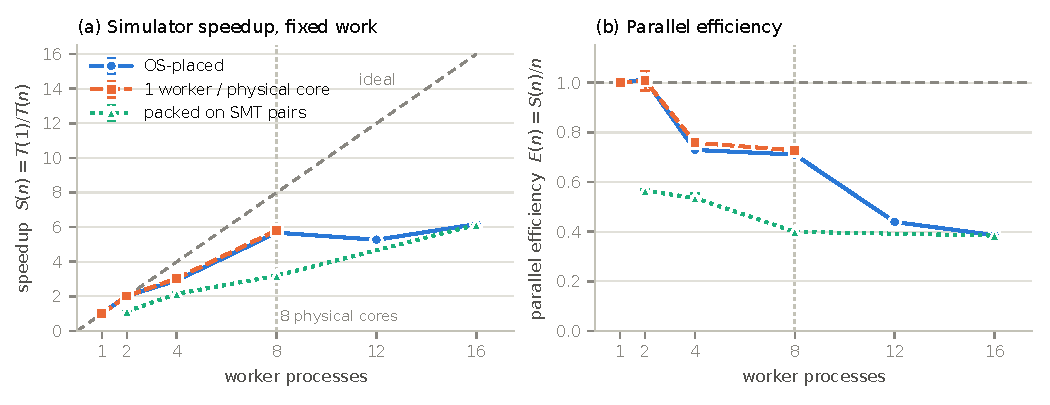
\includegraphics[width=\columnwidth]{fig_hpc_sim.pdf}
\caption{Simulator speedup and parallel efficiency for fixed total work. Dashed lines: ideal.
Bars show bootstrap intervals over repeats. The vertical line marks the 8 physical cores of the
test machine.}
\label{fig:sim}
\end{figure}
One core simulates \NumSimOne{} steps/s, \NumSimDaysPerSecOne{} simulated days per wall-clock
second. With 8 workers the throughput is \NumSimEight{} steps/s (speedup \NumSpeedEight{},
efficiency \NumEffEight{}) and with 16 workers \NumSimSixteen{} steps/s (speedup
\NumSpeedSixteen{}, efficiency \NumEffSixteen{}): scaling flattens at the physical-core count and
hyper-threads add little (Fig.~\ref{fig:sim}). At the highest rate a simulated year takes
\NumYearSeconds{} s.

Placement does not matter here: one worker per physical core and operating-system placement give
the same throughput, packing two workers onto the hyper-thread pair of one core yields only
\NumSmtTwo{}$\times$ the throughput of a single worker, and 16 workers on 8 cores add
\NumSmtGain{}\,\% over 8. Efficiency also falls from about $1$ at two workers to about
$0.75$ at four, with or without pinning, so placement is not the cause. We separated
two further candidates (Fig.~\ref{fig:diag}). Giving every worker identical episodes removes load
imbalance, and the drop persists (the slowest worker takes at most \NumSlowFastSameWork{}$\times$
as long as the fastest). The sampled core clock, however, falls from \NumFreqOneGHz{}\,GHz with one
worker to \NumFreqEightGHz{}\,GHz with eight, tracking the per-worker rate (from \NumPerWorkerOne{} to
\NumPerWorkerEight{} steps/s); rate per GHz changes by a factor of only \NumPerGhzRatioEight{}. We
therefore attribute the efficiency loss to the processor lowering its clock under multi-core
load (the machine runs the \texttt{powersave} governor), not to the parallel decomposition.
This is an inference from one clock reading per worker per run, not a controlled experiment: the
clock could not be fixed on a shared machine.

\begin{figure}[t]
\centering
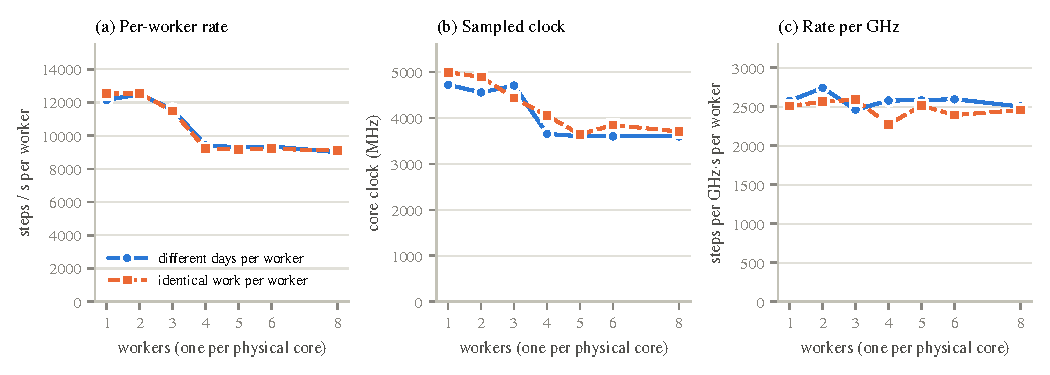
\includegraphics[width=\columnwidth]{fig_hpc_diag.pdf}
\caption{Why efficiency falls between two and four workers. Workers are pinned to distinct
physical cores. (a) Per-worker rate. (b) Core clock, sampled once per worker during the run.
(c) Rate divided by clock. Blue: workers simulate different days; orange: all workers simulate
identical episodes, which removes load imbalance.}
\label{fig:diag}
\end{figure}

\subsection{Learner throughput}
\begin{figure*}[t]
\centering
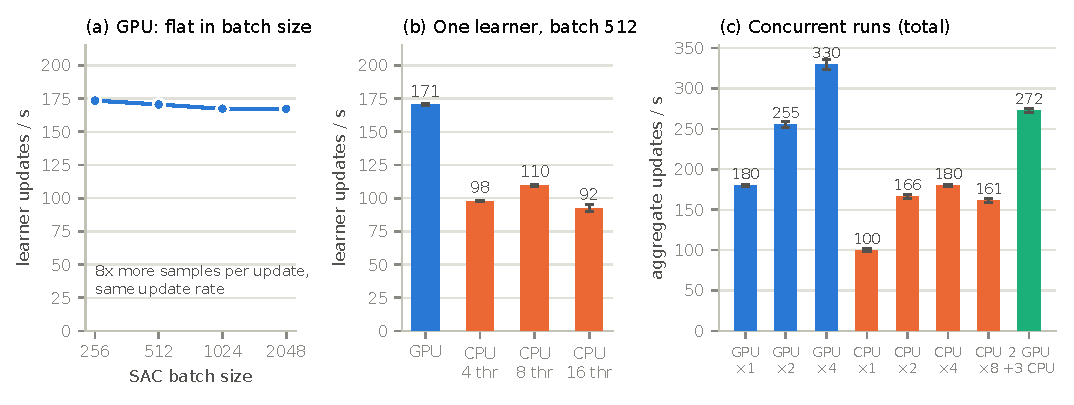
\includegraphics[width=\textwidth]{fig_hpc_learner.pdf}
\caption{SAC learner throughput (updates only; environment stepping excluded). (a) GPU rate is
flat from batch 256 to 2048. (b) One learner, batch 512, by device and CPU thread count.
(c) Total rate of $k$ concurrent runs.}
\label{fig:learner}
\end{figure*}
At a correct update ratio, SAC is limited by the learner, not the simulator: the GPU performs
\NumGpuUps{} updates/s and the rate does not change when the batch grows from 256 to 2048, so
the update is latency-bound, not compute-bound. The CPU performs \NumCpuUpsFour{} updates/s
with 4 threads and \NumCpuUpsEight{} with 8, a GPU advantage of only \NumGpuCpuRatio{}$\times$
(Fig.~\ref{fig:learner}). Because the rate does not depend on the number of environments,
additional environment parallelism does not shorten training.

The remaining lever is running independent runs side by side. On the GPU, one process delivers
\NumMultiGpuOne{} updates/s (one CPU thread per process), two together \NumMultiGpuTwo{} and four
\NumMultiGpuFour{}: aggregate throughput grows, but each process slows down (Fig.~\ref{fig:learner}c).
CPU learners saturate sooner (\NumMultiCpuOne{} updates/s for one 4-thread process,
\NumMultiCpuFour{} for four). Mixing devices is worse than using the GPU alone: two GPU plus three
CPU processes reach only \NumMultiMixed{} updates/s. We did not isolate the cause; a plausible one
is that the CPU learners take cores from the GPU processes' kernel-launch threads. The best configuration we measured
(\NumMultiBestCase{}) gives \NumMultiBest{} updates/s in total.

\subsection{The update-ratio pitfall}
\begin{table}[t]
\caption{Update-to-data ratio of vectorized SAC configurations (Eq.~\ref{eq:utd}).
Measured: SB3 2.9.0, 40\,960 steps with the first configuration; counts are
\texttt{model.\_n\_updates} divided by transitions after the learning-start threshold.}
\label{tab:utd}
\centering
\small
\begin{tabular}{lcccc}
\toprule
$N$ & $F$ & $G$ & documented & measured \\
\midrule
32 & 32 & 32   & 1     & 0.032 \\
32 & 32 & 1024 & ---   & \TODO{rerun to log} \\
\bottomrule
\end{tabular}
\end{table}
A run with the repository configuration performed 992 updates for 30\,960 transitions
(UTD $=0.032$), against a documented ratio of one (Table~\ref{tab:utd}); over $2\times10^6$ steps this is about
\num{62500} updates instead of $\approx 2\times10^6$. An earlier benchmark reported a $26\times$
speedup of this configuration over the library default at ``identical learning dynamics''
(on different hardware; not reproduced here). That order of magnitude is what removing $31/32$ of the
gradient work produces, so the speedup is largely less learning per step, not free
parallelism. Throughput in steps/s should therefore be reported together with the UTD, and
configurations compared by time to a stated quality.

\subsection{Learned controller: pilots at a corrected update ratio}
\begin{table}[t]
\caption{Pilots at $w_2=0.1$, update ratio 1, 300k steps, 32 environments, evaluated on the 293
\emph{training} days (in-sample for the learned policies; the held-out days are not used). Reward is
recomputed from logged components with the original scales and weights; the difference to the
constant-action-$+1$ controller is a per-day mean with a bootstrap interval over days (100 reward
units $=1$\,kg of hydrogen). Days share weather, so the interval describes this day set only.}
\label{tab:pilots}
\centering
\footnotesize
\resizebox{\columnwidth}{!}{% GENERATED by scripts/make_pilot_table.py from grid_round2.csv -- do not edit by hand.
\begin{tabular}{lrrrr}
\toprule
Controller & H$_2$ & $\Delta V$ & trans. & $\Delta$ reward \\
 & [kg/d] & [\si{\micro\volt}/d] & [/d] & vs.\ $+1$ [/d] \\
\midrule
Constant action $+1$ (threshold removed) & 219.6 & 84.9 & 6.0 & --- \\
Tuned slew limit & 214.7 & 80.0 & 7.5 & $-$481 [$-$513, $-$451] \\
Threshold rule (10\,\% idle threshold) & 217.2 & 94.7 & 17.1 & $-$243 [$-$276, $-$211] \\
SAC, $\gamma{=}0.999$, seed 0 & 204.3 & 94.9 & 14.1 & $-$1539 [$-$1598, $-$1481] \\
SAC, $\gamma{=}0.999$, seed 1 & 201.0 & 91.3 & 12.0 & $-$1862 [$-$1929, $-$1795] \\
SAC, $\gamma{=}0.99$, seed 0 & 210.0 & 85.0 & 7.1 & $-$954 [$-$975, $-$932] \\
SAC, $\gamma{=}0.95$, seed 1 & 212.5 & 80.9 & 4.2 & $-$706 [$-$720, $-$691] \\
SAC, $\gamma{=}0.95$, seed 0 & 212.6 & 81.1 & 3.8 & $-$698 [$-$712, $-$684] \\
SAC, $\gamma{=}0.95$, reward$/10$, seed 0 & 212.5 & 80.8 & 3.6 & $-$708 [$-$721, $-$696] \\
SAC, $\gamma{=}0.9$, seed 0 & 212.9 & 80.9 & 3.7 & $-$667 [$-$680, $-$654] \\
SAC, $\gamma{=}0.8$, seed 0 & 212.9 & 80.1 & 3.1 & $-$665 [$-$678, $-$652] \\
\bottomrule
\end{tabular}
% days: 293
}
\end{table}
All pilots train SAC at $w_2=0.1$, a weight at which the best action lies on the boundary of the
action range, with the corrected update ratio (Table~\ref{tab:pilots}). The earlier discount factor
of $0.999$ gave less hydrogen, more degradation and a lower reward than the constant-action rule on
every training day. Lowering $\gamma$ improved every column monotonically down to about $0.95$;
values at or below $0.95$ were indistinguishable, a replicate seed moved the result by about $10$
reward units per day, and rescaling the reward tenfold changed nothing. We read this as the very long
horizon making action differences hard for the critic to resolve; we did not test that directly.
After these corrections SAC still gives up hydrogen for lower degradation and fewer transitions than
the reward at $w_2=0.1$ warrants, and it remains below both the constant-action rule and the tuned
slew limit on every training day. We therefore make no claim that the learned controller improves on
the rule-based ones at this weight. \TODO{E3 (update-ratio study) and E5 (frontier at higher weights,
held-out days) results; text and figures are generated by scripts/analyze\_e3.py and analyze\_e5.py}

\subsection{Sensitivity to resource variability and degradation coefficients}
\begin{figure*}[t]
\centering
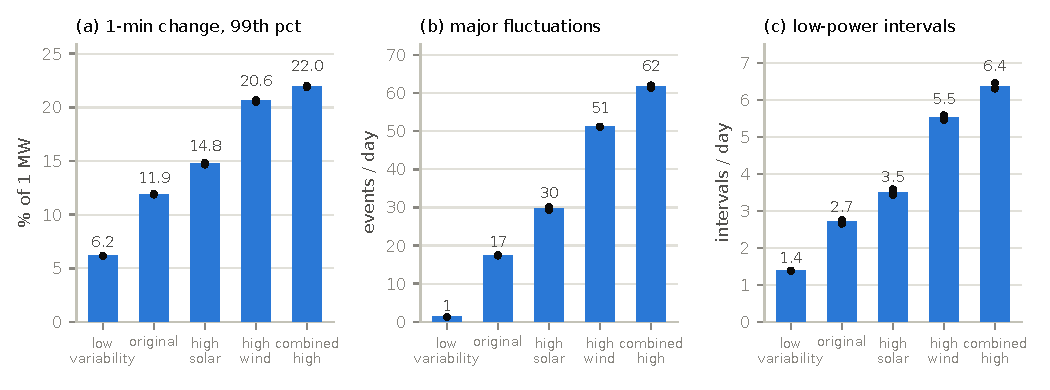
\includegraphics[width=0.92\textwidth]{fig_scenarios.pdf}
\caption{Variability of the five resource scenarios (Section~\ref{sec:scen}). Bars: mean over three
independent noise realisations; dots: individual realisations. ``Major fluctuation'': a ten-minute
change above 20\,\% of \SI{1}{\mega\watt}, consecutive minutes counted once. Capacity factor is
unchanged across scenarios, so differences are due to variability alone. The original scenario is
itself unvalidated against measurements.}
\label{fig:scen}
\end{figure*}
The process-parallel harness (Section~\ref{sec:scen}) evaluated the three rule-based controllers on
the 72 held-out days across \NumVariants{} coefficient variants and the five scenarios with three
realisations each: \NumGridUnits{} simulation units, \NumGridSteps{} environment steps, in
\NumGridSeconds{}\,s on \NumGridWorkers{} workers (\NumGridDaysPerSec{} simulated days per
wall-clock second) while the machine was also running four training jobs. The three rules have no
parameters fitted to those days, except that the slew limit was tuned on training days. Coefficients
were held at their nominal values, which were calibrated on the original profile; this is a
what-if on the resource with the physics fixed, not a recalibration.

\begin{figure*}[t]
\centering
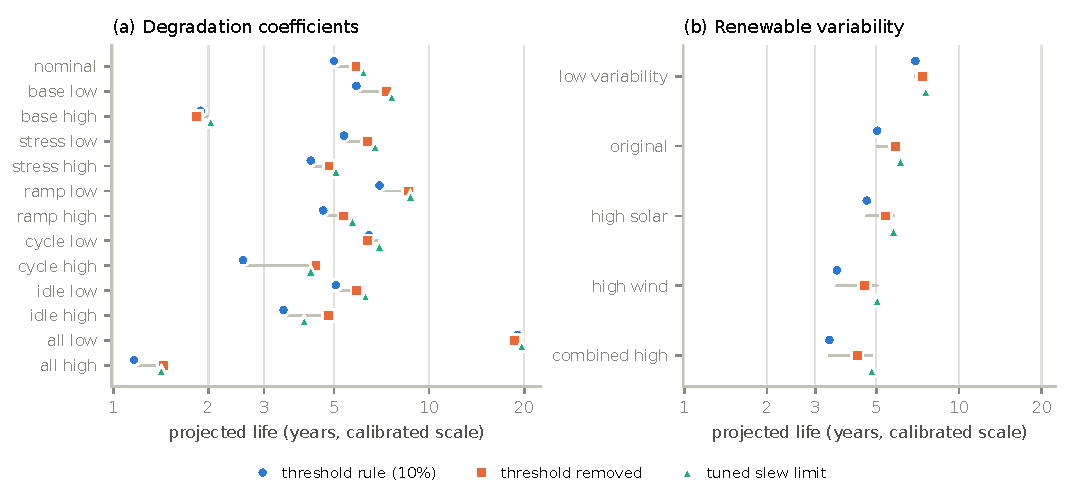
\includegraphics[width=0.92\textwidth]{fig_sensitivity.pdf}
\caption{Projected life of the three rule-based controllers (a) under each degradation coefficient set
at its lower and upper literature-interval bound, one at a time, and jointly, and (b) across the
resource scenarios at nominal coefficients. Life uses the model's calibrated scale (end of life at
\SI{177}{\milli\volt} rise), not a physical lifetime.}
\label{fig:sens}
\end{figure*}
Uncertainty in the degradation coefficients dominates. For the published rule, projected life
ranges from \NumLifeMin{} to \NumLifeMax{} years across the variants, a factor of \NumLifeSpread{},
whereas at nominal coefficients the three controllers differ by tens of percent (\NumLifeNominalNaive{},
\NumLifeNominalNoThr{} and \NumLifeNominalRamp{} years for the published rule, the rule without its
threshold, and the slew-limited rule). Hydrogen yield ranks the controllers identically in every
variant and scenario, with a spread of at most \NumScenHydrogenSpreadPct{}\,\% between controllers in any
scenario. The lifetime ordering is also identical across the five variability scenarios, but it
changes in \NumRankFlips{} of the \NumVariants{} coefficient variants: for example, removing the threshold
gives the longest life when the cost per on/off transition is high, and the shortest when
that cost or the base rate is low. A conclusion about which of these controllers is best for stack
life therefore depends on coefficients the model cannot pin down. Resource variability matters
as well: the published rule's projected life falls from \NumScenLifeMax{} years in the low-variability
scenario to \NumScenLifeMin{} in the combined-high scenario. \TODO{add the learned policies to this
comparison once a candidate is selected}

% =============================================================================
\section{Limitations}\label{sec:limits}
\emph{No hardware validation.} No stack was operated; the plant model is parameterised from published
ranges and the degradation model is calibrated to literature-reported rates. We claim neither
absolute lifetimes nor transfer of controller rankings to hardware. \emph{Variability is
synthetic.} The one-minute resource structure is generated; the default amplitudes imply a
99th-percentile one-minute change of about $12\%$ of capacity, which we have not checked
against measurements. The scenarios bound sensitivity to the assumption but do not validate it.
\emph{Physical consistency.} With the model's own crossover parameters, hydrogen in the anode gas
exceeds the usual $4$\,vol\% flammability reference below about
\SI{0.8}{\ampere\per\centi\meter\squared}, which includes the efficiency peak; either the
crossover is too high for a real stack or the low-load region is not operable. We have not
changed the model. \emph{Scale.} All measurements are from one workstation with 8 physical
cores and one GPU; we make no claim about larger systems. \emph{Statistics.} Repeats of a
benchmark characterise one machine, not a population. \emph{Single site and year.}

% =============================================================================
\section{Conclusion}
\TODO{write after E3--E6: three or four sentences, each tied to a measured result; state what the
controller comparison does and does not show; hardware validation as future work.}

\bibliographystyle{IEEEtran}
\bibliography{refs}

\end{document}
